% !TEX root = ../tex/3-2.tex
% 第3章：本文は青、補足は緑
\newcommand{\asmain}{%
    \setbeamercolor{frametitle}{fg=white,bg=main}%
    \setbeamercolor{structure}{fg=main}%
    \setbeamercolor{itemize item}{fg=main}%
    \setbeamercolor{itemize subitem}{fg=main}%
    \setbeamercolor{enumerate item}{fg=main}%
}
\newcommand{\assuppl}{%
    \setbeamercolor{frametitle}{fg=white,bg=examplecol}%
    \setbeamercolor{structure}{fg=examplecol}%
    \setbeamercolor{itemize item}{fg=examplecol}%
    \setbeamercolor{itemize subitem}{fg=examplecol}%
    \setbeamercolor{enumerate item}{fg=examplecol}%
}
\asmain


%=============================================
\begin{frame}{3.1から3.2へ}
    \begin{block}{ここまで（3.1）}
        EBMはエネルギー$E_\phi$で分布を表し、
        スコア$s_\phi=-\nabla_{\bm{x}}E_\phi$で生成できる。\\
        スコアマッチングは分配関数を避けるが、
        エネルギー経由だと二階微分が残る。
    \end{block}
    \begin{block}{ここから（3.2）}
        ランジュバン動力学に必要なのはスコアだけである。\\
        だからエネルギーを経由せず、
        ニューラルネットでスコアを直接学習する。
    \end{block}
    \begin{itemize}
        \item エネルギーをモデル化する $\;\to\;$ スコアをモデル化する
        \item この転換が、スコアベース生成モデルの土台になる
    \end{itemize}
\end{frame}
%=============================================
\asmain
\begin{frame}{3.2 の位置づけ}
    \begin{block}{この節の役割}
        EBMのスコア視点から、スコアを直接扱う生成モデルへ橋を渡す
    \end{block}
    \begin{enumerate}
        \item \textbf{3.2.1 スコアマッチングによる学習}\\
        真のスコアへ当てはめる損失と、
        真のスコアなしで使える等価形
        \item \textbf{3.2.2 ランジュバン動力学によるサンプリング}\\
        学習したスコア$s_{\phi^\star}$でサンプルを得る
        \item \textbf{3.2.3 予告：スコアベース生成モデル}\\
        この章の後半（DSM / NCSN）へのつながり
    \end{enumerate}
\end{frame}
%=============================================
\section{3.2.1 スコアマッチングによる学習}
\asmain
\begin{frame}{区切り：3.2.1 スコアマッチングによる学習}
    \tableofcontents[currentsection]
\end{frame}
%=============================================
\asmain
\begin{frame}{スコアをニューラルネットで直接近似する}
    データ分布のスコア
    \[
        s(\bm{x})
        =
        \nabla_{\bm{x}}\log p_{\mathrm{data}}(\bm{x})
    \]
    を、ベクトル場としてパラメータ化したネット
    $s_\phi(\bm{x})$で近似する。
    \[
        s_\phi(\bm{x})\;\approx\;s(\bm{x})
    \]
    \begin{block}{3.1との違い}
        3.1では$s_\phi=-\nabla_{\bm{x}}E_\phi$と、エネルギー経由でスコアを得た。\\
        ここでは$s_\phi$そのものを学習対象にする。
    \end{block}
\end{frame}
%=============================================
\asmain
\begin{frame}{図3.4：スコアマッチングのイメージ}
    \centering
    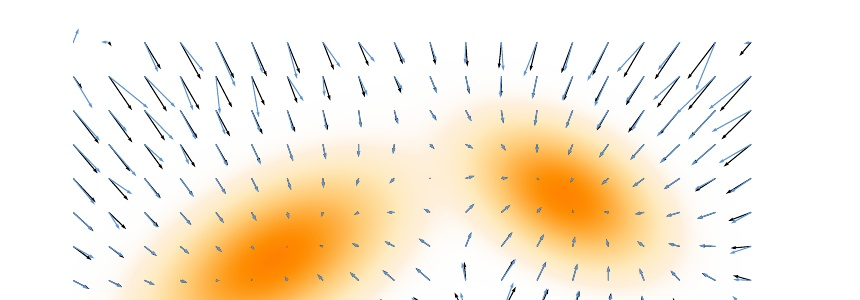
\includegraphics[width=\textwidth,height=0.68\textheight,keepaspectratio]{fig-3-4.jpg}
    \vfill
    ニューラルネットのスコア$s_\phi(\bm{x})$を、
    真のスコア$s(\bm{x})$にMSEで合わせる。\\
    どちらもベクトル場として表される。
\end{frame}
%=============================================
\assuppl
\begin{frame}{\supplmark：図3.4の読み方}
    \begin{exampleblock}{オレンジの領域}
        データの高密度領域（モード）である。
        スコアはここに向かう向きをもつ。
    \end{exampleblock}
    \begin{exampleblock}{矢印}
        各点でのスコアベクトルである。\\
        真の場$s$とモデルの場$s_\phi$を重ねて描き、
        MSEで一致させるイメージである。
    \end{exampleblock}
    \begin{exampleblock}{学習の目標}
        どこで密度が増えるかを、
        エネルギー関数を経由せずにベクトル場として覚える。
    \end{exampleblock}
\end{frame}
%=============================================
\asmain
\begin{frame}{スコアを合わせる損失}
    真のスコアとモデルのスコアの平均二乗誤差を最小化する。
    \[
        \mathcal{L}_{\mathrm{SM}}(\phi)
        :=
        \frac12
        \mathbb{E}_{\bm{x}\sim p_{\mathrm{data}}}
        \bigl[
        \|s_\phi(\bm{x})-s(\bm{x})\|_2^2
        \bigr]
        \tag{3.2.1}
    \]
    \begin{block}{一見すると使えない}
        回帰の教師$s(\bm{x})=\nabla_{\bm{x}}\log p_{\mathrm{data}}(\bm{x})$が未知である。\\
        観測できるのはサンプルだけで、真の密度もスコアも通常はわからない。
    \end{block}
\end{frame}
%=============================================
\asmain
\begin{frame}{命題3.2.1：Hyv\"arinenの扱いやすい形}
    \[
        \mathcal{L}_{\mathrm{SM}}(\phi)
        =
        \mathcal{L}_{\mathrm{eSM}}(\phi)+C
    \]
    ここで
    \[
        \resizebox{0.98\textwidth}{!}{$
        \mathcal{L}_{\mathrm{eSM}}(\phi)
        :=
        \mathbb{E}_{\bm{x}\sim p_{\mathrm{data}}}
        \Bigl[
        \operatorname{Tr}\bigl(\nabla_{\bm{x}}s_\phi(\bm{x})\bigr)
        +
        \tfrac12\|s_\phi(\bm{x})\|_2^2
        \Bigr]
        $}
        \tag{3.2.2}
    \]
    であり、$C$は$\phi$に依らない定数である。\\
    最小化の解は$s^\star(\cdot)=\nabla_{\bm{x}}\log p(\cdot)$である。
\end{frame}
%=============================================
\assuppl
\begin{frame}{なぜ真のスコアが消えるか（狙い）}
    式（3.2.1）の教師$s=\nabla\log p_{\mathrm{data}}$は未知である。\\
    付録D.2.1では、二乗を展開し部分積分でクロス項の微分をモデル側へ移す。
    \begin{exampleblock}{残るもの}
        モデルの大きさ$\|s_\phi\|_2^2$と、
        ヤコビアンの対角和$\operatorname{Tr}(\nabla_{\bm{x}}s_\phi)$だけ。\\
        データサンプル上の平均で評価できる$\Rightarrow$式（3.2.2）。
    \end{exampleblock}
    \begin{exampleblock}{3.1との違い}
        3.1はエネルギー経由でヘッセが出た。\\
        ここでは$s_\phi$を直接パラメータ化するので、トレースが残る。
    \end{exampleblock}
\end{frame}
%=============================================
\assuppl
\begin{frame}{\supplmark：D.2.1①　二乗を展開する}
    \[
        \resizebox{0.98\textwidth}{!}{$
        \mathcal{L}_{\mathrm{SM}}(\phi)
        =
        \dfrac12
        \mathbb{E}_{p_{\mathrm{data}}}
        \bigl[
        \|s_\phi\|_2^2
        -
        2\langle s_\phi,\,s\rangle
        +
        \|s\|_2^2
        \bigr]
        $}
    \]
    すなわち
    \[
        \resizebox{0.98\textwidth}{!}{$
        \mathcal{L}_{\mathrm{SM}}
        =
        \dfrac12\mathbb{E}[\|s_\phi\|_2^2]
        -
        \mathbb{E}[\langle s_\phi,\,s\rangle]
        +
        \dfrac12\mathbb{E}[\|s\|_2^2].
        $}
    \]
    最後の項は$p_{\mathrm{data}}$だけで決まり$\phi$に依らない（定数$C$の一部）。
\end{frame}
%=============================================
\assuppl
\begin{frame}{\supplmark：D.2.1②　クロス項で$p$が約分される}
    $s=\nabla_{\bm{x}}\log p_{\mathrm{data}}=\nabla p_{\mathrm{data}}/p_{\mathrm{data}}$より
    \[
        \mathbb{E}[\langle s_\phi,\,s\rangle]
        =
        \int s_\phi(\bm{x})^{\top}
        \nabla_{\bm{x}}p_{\mathrm{data}}(\bm{x})\,d\bm{x}.
    \]
    座標成分ごとに書くと
    \[
        \sum_{i=1}^{D}
        \int
        s_\phi^{(i)}(\bm{x})\,
        \partial_{x_i}p_{\mathrm{data}}(\bm{x})\,
        d\bm{x}.
    \]
\end{frame}
%=============================================
\assuppl
\begin{frame}{\supplmark：D.2.1③　部分積分で微分をモデルへ}
    各$i$で$u=s_\phi^{(i)}$、$v=p_{\mathrm{data}}$として部分積分し、
    境界で$|uv|\to0$（$R\to\infty$）を仮定する。
    \[
        \int s_\phi^{(i)}\,\partial_{x_i}p_{\mathrm{data}}
        =
        -
        \int
        (\partial_{x_i}s_\phi^{(i)})\,
        p_{\mathrm{data}}.
    \]
    $i$について和をとると
    \[
        \mathbb{E}[\langle s_\phi,\,s\rangle]
        =
        -
        \mathbb{E}\bigl[
        \operatorname{Tr}(\nabla_{\bm{x}}s_\phi)
        \bigr].
    \]
\end{frame}
%=============================================
\assuppl
\begin{frame}{\supplmark：D.2.1④　$\mathcal{L}_{\mathrm{SM}}=\mathcal{L}_{\mathrm{eSM}}+C$}
    クロス項の符号を戻すと
    \[
        \resizebox{0.98\textwidth}{!}{$
        \mathcal{L}_{\mathrm{SM}}(\phi)
        =
        \mathbb{E}_{p_{\mathrm{data}}}
        \Bigl[
        \operatorname{Tr}(\nabla_{\bm{x}}s_\phi)
        +
        \tfrac12\|s_\phi\|_2^2
        \Bigr]
        +
        C
        $}
    \]
    括弧内が$\mathcal{L}_{\mathrm{eSM}}$（式3.2.2）。\\
    $C=\tfrac12\mathbb{E}[\|s\|_2^2]$は$\phi$に依らない。
\end{frame}
%=============================================
\asmain
\begin{frame}{式（3.2.2）の二つの項──これから図で見る}
    \[
        \mathcal{L}_{\mathrm{eSM}}(\phi)
        =
        \mathbb{E}_{p_{\mathrm{data}}}
        \Bigl[
        \underbrace{\operatorname{Tr}(\nabla_{\bm{x}}s_\phi)}_{\text{発散項}}
        +
        \underbrace{\tfrac12\|s_\phi\|_2^2}_{\text{大きさの項}}
        \Bigr]
    \]
    \begin{itemize}
        \item \textbf{大きさの項}: $\|s_\phi\|^2$ を抑える罰則。\\
        期待値が$p_{\mathrm{data}}$なので\textbf{データの多い場所ほど強く効く}。
        \item \textbf{発散項}: 正の符号で入るので、最小化は\textbf{局所収縮}を好む。
        \item 最適解$s^\star=\nabla\log p_{\mathrm{data}}$になる理由は、後で SM と同値性から示す。
    \end{itemize}
\end{frame}
%=============================================
\asmain
\begin{frame}{図解：大きさの項は高密度ほど重い}
    \centering
    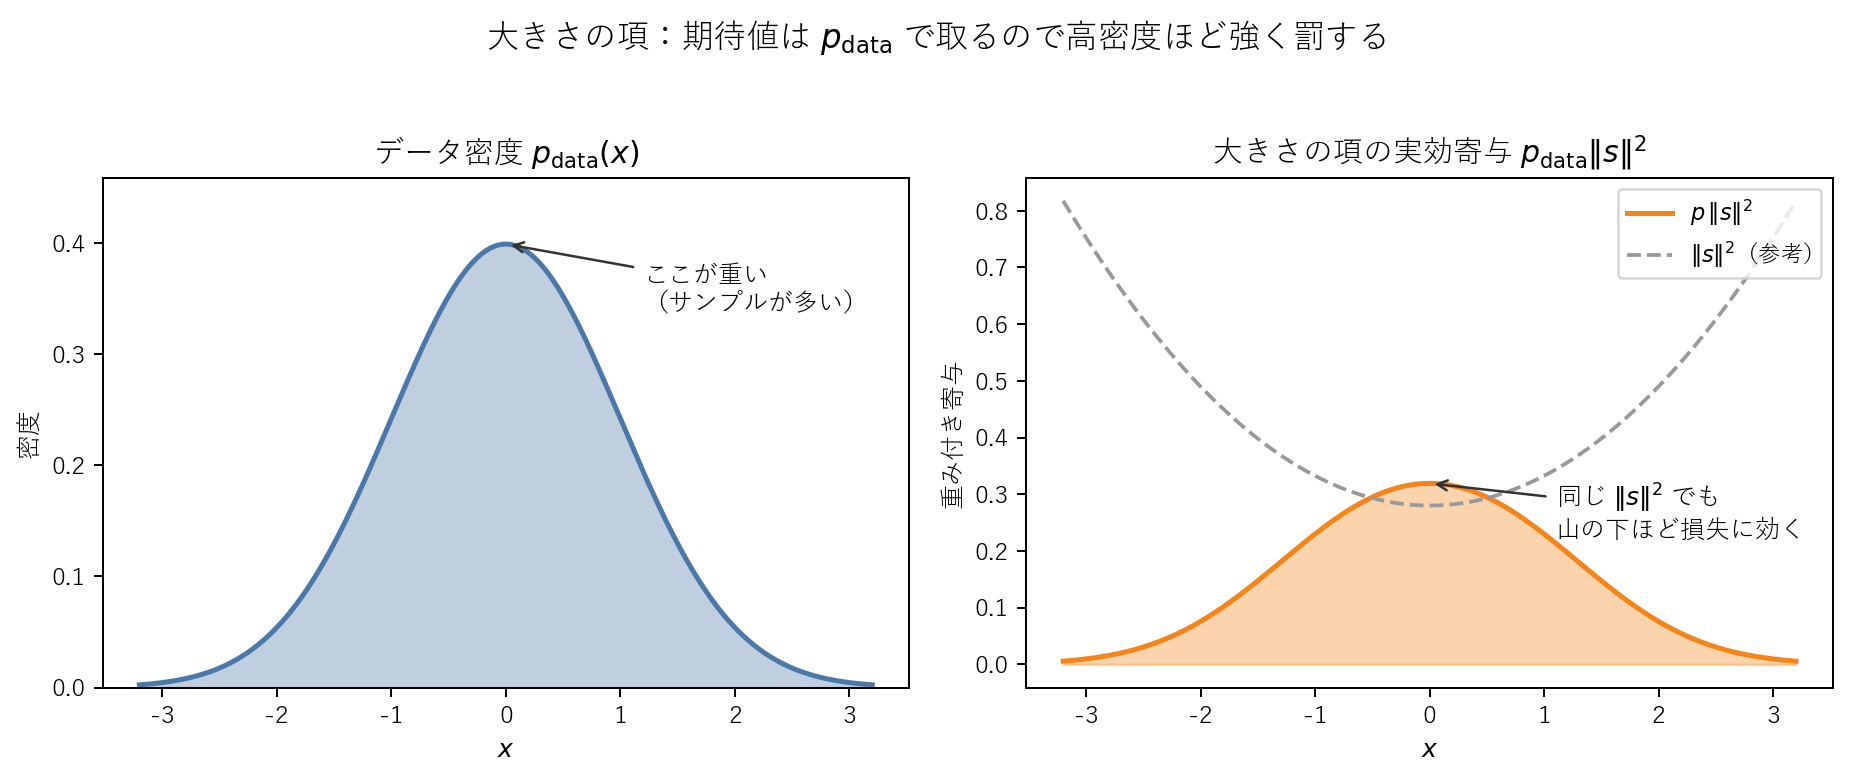
\includegraphics[width=0.95\linewidth]{esm-magnitude.png}
    \vspace{-0.3em}
    \begin{exampleblock}{一文}
        同じ$\|s\|^2$でも、$p_{\mathrm{data}}$が大きい場所の寄与が損失を支配する。
    \end{exampleblock}
\end{frame}
%=============================================
\asmain
\begin{frame}{図解：なぜ「データが多いと強く効く」のか}
    期待値の定義どおり
    \[
        \mathbb{E}_{p_{\mathrm{data}}}\!\bigl[\tfrac12\|s_\phi\|^2\bigr]
        =\int p_{\mathrm{data}}(\bm{x})\,\tfrac12\|s_\phi(\bm{x})\|_2^2\,\mathrm{d}\bm{x}.
    \]
    \begin{columns}[T,onlytextwidth]
        \begin{column}{0.52\textwidth}
            \begin{block}{イメージ}
                積分は「各地点の罰則$\times$そこにいる確率」。\\
                人が多い駅では、同じマナー違反でも影響が大きい、に近い。
            \end{block}
        \end{column}
        \begin{column}{0.46\textwidth}
            \begin{exampleblock}{誤解しやすい点}
                高密度の\textbf{すべての点}で$s_\phi=0$にはならない。\\
                最適$s^\star=\nabla\log p$がゼロなのは、密度の頂上（停留点）だけ。
            \end{exampleblock}
        \end{column}
    \end{columns}
\end{frame}
%=============================================
\asmain
\begin{frame}{図解：発散項は収縮（吸い込み）を好む}
    \centering
    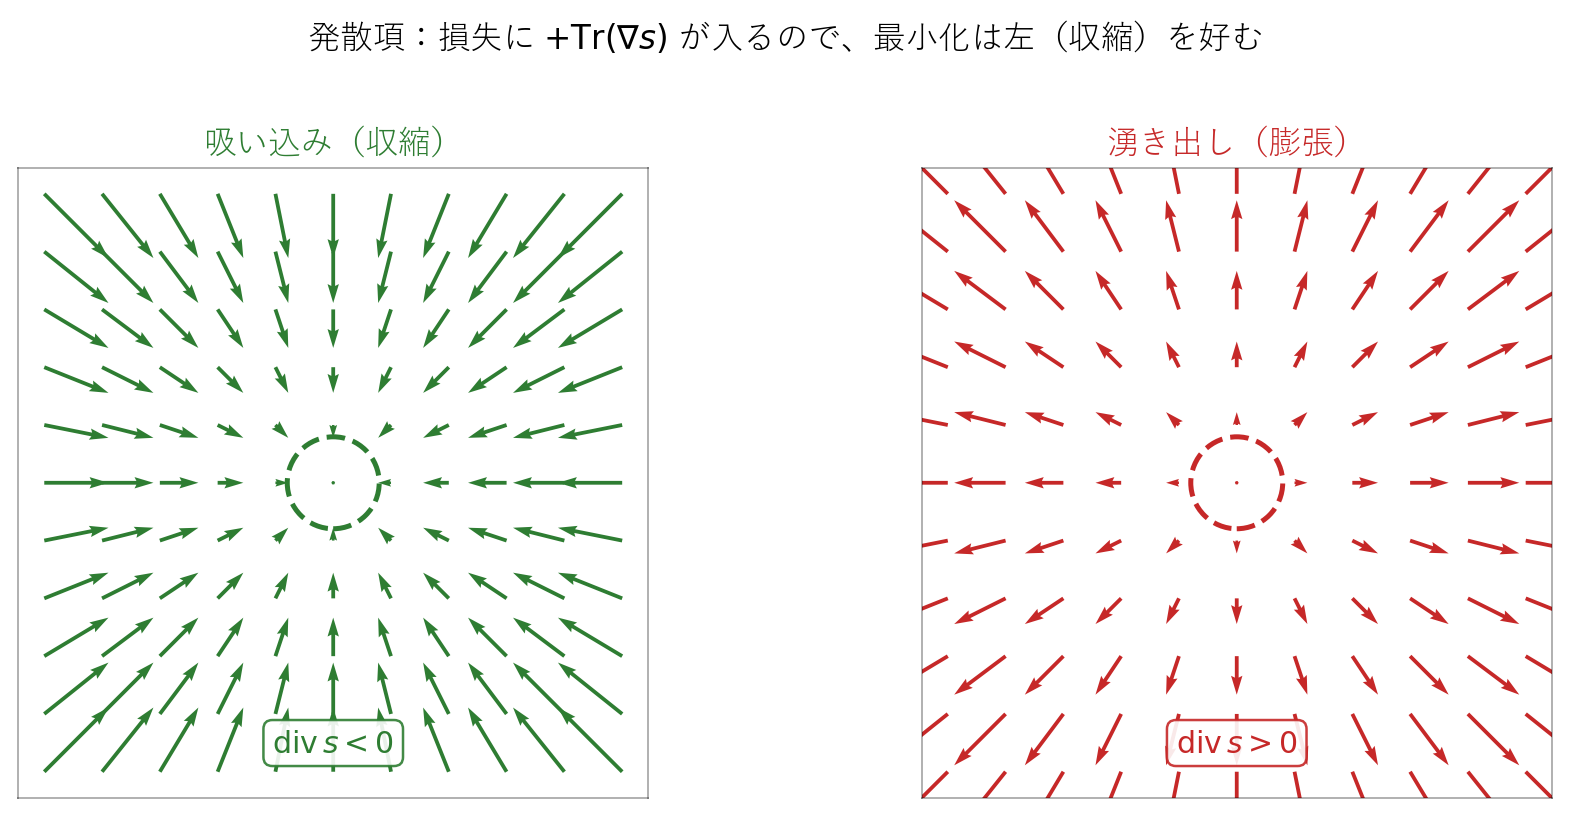
\includegraphics[width=0.92\linewidth]{esm-divergence.png}
    \vspace{-0.2em}
    \begin{block}{読み方}
        損失に$+\operatorname{Tr}(\nabla s)$が入る $\Rightarrow$
        発散が正（湧き出し）だと損、負（吸い込み）だと得。\\
        だから最小化は左の場を好む。
    \end{block}
\end{frame}
%=============================================
\asmain
\begin{frame}{凹性：場が（近似的に）勾配のとき}
    発散項は正符号なので、最小化は\textbf{負の発散}（局所収縮）を好む。\\
    ただし負の発散だけでは、停留点が吸い込みだと\textbf{保証しない}。
    \begin{block}{精密化のための仮定}
        対数密度に合わせる設定では自然なので、
        スカラー$u:\mathbb{R}^D\to\mathbb{R}$に対し$s_\phi=\nabla_{\bm{x}}u$とおく。
        \[
            \nabla_{\bm{x}}s_\phi=\nabla_{\bm{x}}^2 u
            \quad\text{（ヘッセ）},\qquad
            \operatorname{Tr}(\nabla_{\bm{x}}s_\phi)
            =\operatorname{Tr}(\nabla_{\bm{x}}^2 u)
            \quad\text{（発散）}.
        \]
    \end{block}
\end{frame}
%=============================================
\asmain
\begin{frame}{凹性：停留点での2次近似}
    停留点$\bm{x}^\star$（$s_\phi(\bm{x}^\star)=\nabla_{\bm{x}}u(\bm{x}^\star)=0$）では
    \[
        u(\bm{x})
        =
        u(\bm{x}^\star)
        +
        \tfrac12
        (\bm{x}-\bm{x}^\star)^\top
        \nabla_{\bm{x}}^2 u(\bm{x}^\star)
        (\bm{x}-\bm{x}^\star)
        +
        o(\|\bm{x}-\bm{x}^\star\|_2^2).
    \]
    ヘッセ$\nabla_{\bm{x}}^2 u(\bm{x}^\star)$が\textbf{負定値}なら、
    $u$は$\bm{x}^\star$で局所凹であり、対数密度はそこで厳密な局所最大になる。
\end{frame}
%=============================================
\asmain
\begin{frame}{凹性：負定値なら吸い込みになる}
    ヘッセの固有値がすべて負 $\Rightarrow$
    $\operatorname{Tr}(\nabla_{\bm{x}}^2 u(\bm{x}^\star))<0$。
    \begin{block}{結論}
        この場合、停留点はスコア場の下で\textbf{局所的に吸引的}である。\\
        小さな摂動は$\bm{x}^\star$へ引き戻される（吸い込み）。
    \end{block}
    \begin{itemize}
        \item 負の発散を好むこと（損失の符号）
        \item 勾配場$+$負定値ヘッセ $\Rightarrow$ 局所凹・局所最大・吸引
    \end{itemize}
\end{frame}
%=============================================
\assuppl
\begin{frame}{\supplmark：負のトレースだけでは足りない}
    厳密な凹性（したがって対数密度の厳密な局所最大）には、
    ヘッセ$\nabla_{\bm{x}}^2 u$全体が負定値であることが必要で、
    単にトレースが負なだけでは足りない。
    \begin{exampleblock}{逆は成り立たない}
        トレースが負でも、正の固有値が混ざれば鞍点になり得る。\\
        したがって「発散が負 $\Rightarrow$ 必ず局所最大」ではない。
    \end{exampleblock}
    \begin{exampleblock}{読み方}
        発散項は収縮を促す項であり、単独でモードの形を保証する条件ではない。
    \end{exampleblock}
\end{frame}
%=============================================
\asmain
\begin{frame}{なぜ最適解が$s^\star=\nabla\log p_{\mathrm{data}}$なのか}
    \centering
    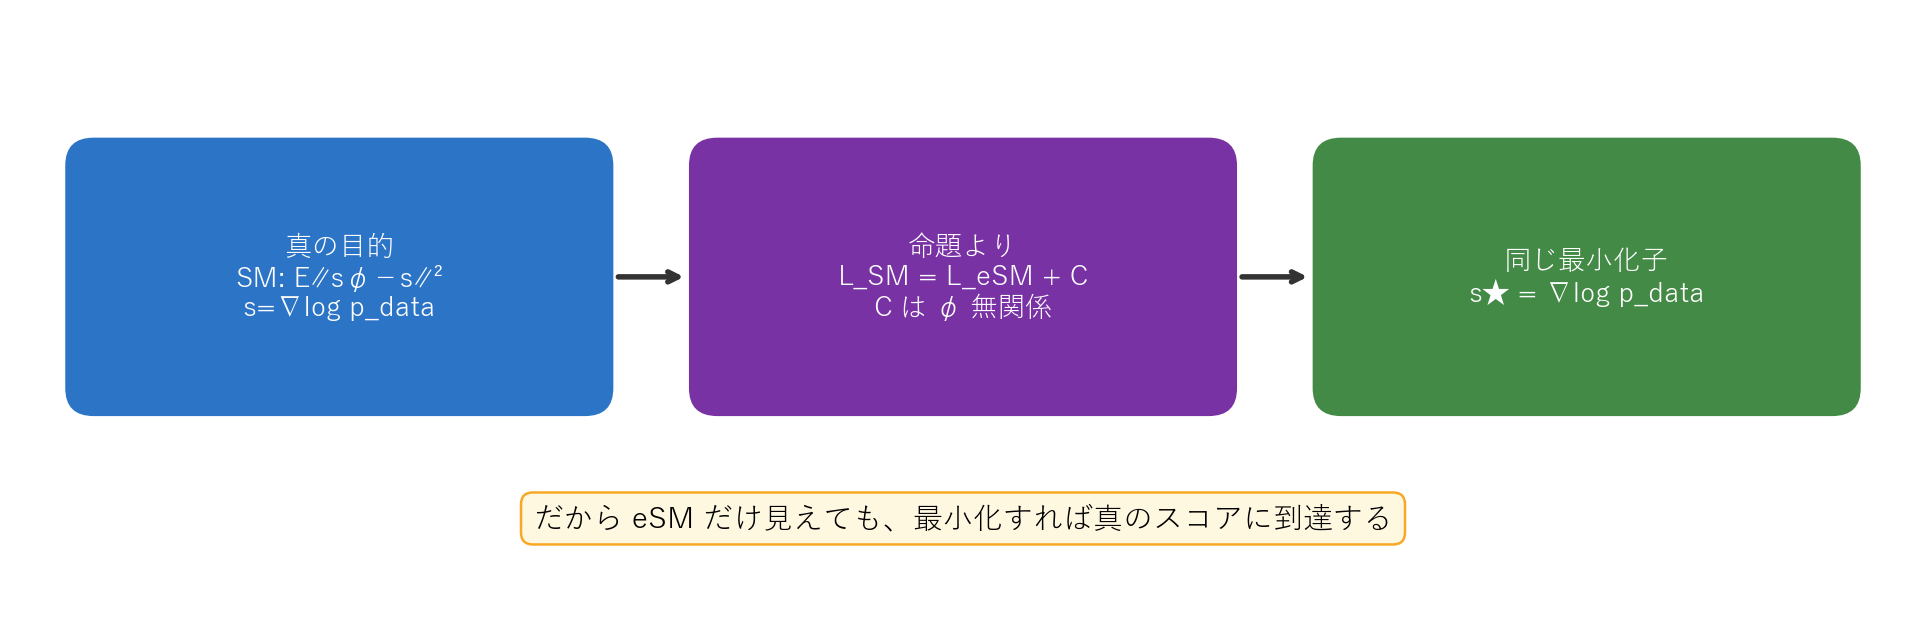
\includegraphics[width=0.96\linewidth]{esm-why-optimal.png}
\end{frame}
%=============================================
\asmain
\begin{frame}{最適性の道筋（数式）}
    \begin{enumerate}
        \item 出発点は真の SM:
        $\displaystyle
        \mathcal{L}_{\mathrm{SM}}(\phi)
        =\tfrac12\mathbb{E}_{p_{\mathrm{data}}}\|s_\phi-s\|_2^2$,\quad
        $s=\nabla\log p_{\mathrm{data}}$.
        \item 命題3.2.1より
        $\mathcal{L}_{\mathrm{SM}}(\phi)=\mathcal{L}_{\mathrm{eSM}}(\phi)+C$
        （$C$は$\phi$無関係）。
        \item したがって\textbf{同じ最小化子}を共有する。\\
        SM の最小は$s_\phi=s$なので、eSM も
        $s^\star=\nabla_{\bm{x}}\log p_{\mathrm{data}}$。
    \end{enumerate}
    \begin{block}{二つの項の役割（直感）}
        大きさの項はノルムを抑え、発散項は密度の形に合わせる。\\
        両者が釣り合う点が真のスコア場である。
    \end{block}
\end{frame}
%=============================================
\assuppl
\begin{frame}{インタラクティブ：場を切り替えて損失を見る}
    ブラウザで次を開くと、吸い込み／湧き出し／真のスコアを切り替え、
    発散の色と大きさの項の効きをその場で比較できる。
    \begin{block}{ファイル}
        \texttt{ch03-score-ncsn/3-2/interactive/esm-intuition.html}
    \end{block}
    \begin{itemize}
        \item 「湧き出し」→ 発散項が正で損失が悪化
        \item 「大きすぎる場」→ ノルム罰が跳ね上がる
        \item 「真のスコア」→ バランスが取れる
    \end{itemize}
\end{frame}
%=============================================
\asmain
\begin{frame}{3.2.1 のまとめ}
    \begin{itemize}
        \item スコア$s_\phi$をニューラルネットで直接近似する
        \item MSE損失（3.2.1）の教師は未知だが、
        等価形（3.2.2）はデータとモデルだけで評価できる
        \item \textbf{大きさの項}: $p_{\mathrm{data}}$で重み付けされた$\|s\|^2$の罰則
        \item \textbf{発散項}: 正符号のため収縮（吸い込み）を好む
        \item \textbf{凹性}: 勾配場でヘッセが負定値なら局所最大・吸引
        \item SM$=$eSM$+C$なので最適は$s^\star=\nabla\log p_{\mathrm{data}}$
    \end{itemize}
    \begin{block}{次}
        学習した$s_{\phi^\star}$を、ランジュバン動力学に入れてサンプルする。
    \end{block}
\end{frame}
%=============================================
\section{3.2.2 ランジュバン動力学によるサンプリング}
\asmain
\begin{frame}{区切り：3.2.2 ランジュバン動力学によるサンプリング}
    \tableofcontents[currentsection]
\end{frame}
%=============================================
\asmain
\begin{frame}{学習したスコアでランジュバン更新する}
    式（3.2.2）を最小化して得た$s_{\phi^\star}$を、
    ランジュバン動力学のスコアとして使う。
    \[
        \bm{x}_{n+1}
        =
        \bm{x}_n
        +
        \eta\,s_{\phi^\star}(\bm{x}_n)
        +
        \sqrt{2\eta}\,\bm{\epsilon}_n,
        \qquad
        \bm{\epsilon}_n\sim\mathcal{N}(\bm{0},\bm{I})
        \tag{3.2.3}
    \]
    $\bm{x}_0$から始め、$n=0,1,2,\ldots$と更新する。
    \begin{block}{3.1との対応}
        EBMでは$s_\phi=-\nabla_{\bm{x}}E_\phi$を入れた式（3.1.5）だった。\\
        ここではエネルギーを持たず、$s_{\phi^\star}$をそのまま入れる。
    \end{block}
\end{frame}
%=============================================
\asmain
\begin{frame}{連続時間ではSDEになる}
    式（3.2.3）は、次のランジュバンSDEの
    オイラー・丸山離散化である。
    \[
        d\bm{x}(t)
        =
        s_{\phi^\star}(\bm{x}(t))\,dt
        +
        \sqrt{2}\,d\bm{w}(t)
    \]
    $\bm{w}(t)$は標準ブラウン運動である。
    \begin{itemize}
        \item ステップ幅$\eta$が小さい極限では、離散更新と連続SDEは一致する
        \item 実装では離散サンプラを走らせても、SDEを直接シミュレートしてもよい
    \end{itemize}
    \begin{block}{要点}
        学習の出力はスコア場であり、
        生成はその場に沿った確率的な流れである。
    \end{block}
\end{frame}
%=============================================
\assuppl
\begin{frame}{\supplmark：更新の二つの働き}
    \[
        \bm{x}_{n+1}
        =
        \bm{x}_n
        +
        \underbrace{\eta\,s_{\phi^\star}(\bm{x}_n)}_{\text{スコア方向へ進む}}
        +
        \underbrace{\sqrt{2\eta}\,\bm{\epsilon}_n}_{\text{探索のためのノイズ}}
    \]
    \begin{exampleblock}{ドリフト}
        学習したスコアに従い、密度が高い方向へ動かす。
    \end{exampleblock}
    \begin{exampleblock}{拡散}
        勾配だけでは局所に止まり得る。
        ノイズが別の領域を探る余地を作る。
    \end{exampleblock}
    詳細な定常分布や混合の議論は3.1.4と同じ骨格である。
\end{frame}
%=============================================
\asmain
\begin{frame}{3.2.2 のまとめ}
    \begin{itemize}
        \item 学習後の$s_{\phi^\star}$を式（3.2.3）に入れればサンプルできる
        \item 連続時間では$d\bm{x}=s_{\phi^\star}\,dt+\sqrt{2}\,d\bm{w}$
        \item エネルギー関数を保持しなくても、スコア場だけで生成できる
    \end{itemize}
\end{frame}
%=============================================
\section{3.2.3 予告：スコアベース生成モデル}
\asmain
\begin{frame}{区切り：3.2.3 予告：スコアベース生成モデル}
    \tableofcontents[currentsection]
\end{frame}
%=============================================
\asmain
\begin{frame}{スコアが拡散モデルの中心になる}
    スコアは当初、EBMを効率よく学習するための道具だった。
    いまでは、スコアそのものが生成モデルの中核になっている。
    \begin{block}{この章の後半で見ること}
        スコア関数が、スコアベース拡散モデルの理論と実装をどう支えるか。\\
        確率過程を通じたデータ生成の枠組みへ進む。
    \end{block}
    \begin{itemize}
        \item 単一ノイズでのスコア学習（Denoising Score Matching）
        \item 複数ノイズへの拡張（NCSN）
        \item DDPMとの対応
    \end{itemize}
\end{frame}
%=============================================
\assuppl
\begin{frame}{\supplmark：いまの枠組みに残る課題}
    式（3.2.2）は真のスコアを消すが、
    $\operatorname{Tr}(\nabla_{\bm{x}}s_\phi)$の計算は高次元で重い。
    \begin{exampleblock}{次の節への動機}
        \begin{itemize}
            \item スライスド・スコアマッチング：
            ランダム方向でトレースを推定する
            \item Denoising Score Matching：
            既知ノイズの条件付きスコアを教師にする
        \end{itemize}
        どちらも「生の$p_{\mathrm{data}}$のスコアを直接扱う」難しさを避ける方向である。
    \end{exampleblock}
\end{frame}
%=============================================
\asmain
\begin{frame}{3.2 全体のまとめ}
    \begin{enumerate}
        \item \textbf{転換}
        生成に必要なのはスコアなので、
        エネルギーではなく$s_\phi$を直接学習する。
        \item \textbf{学習}
        MSE（3.2.1）は教師が未知だが、
        等価形（3.2.2）でデータから学習できる。
        \item \textbf{生成}
        学習した$s_{\phi^\star}$をランジュバン動力学（3.2.3）に入れる。
        \item \textbf{次へ}
        トレース計算や多様体上の不安定さを避けるため、
        DSMと多ノイズのNCSNへ進む。
    \end{enumerate}
\end{frame}
%=============================================
\asmain
\begin{frame}{3.2 全体のまとめ：一本の流れ}
    \begin{block}{今日の道筋}
        EBMではスコアで足りる
        $\;\to\;$
        スコアをネットで直接近似する
        $\;\to\;$
        等価なスコアマッチングで学習する
        $\;\to\;$
        ランジュバンで生成する
    \end{block}
    \begin{block}{核心}
        密度やエネルギーを経由せず、
        対数密度の勾配（スコア）をベクトル場として学べばよい。
    \end{block}
    \begin{block}{次へ}
        3.3では、ノイズを入れた条件付きスコア学習
        （Denoising Score Matching）を扱う。
    \end{block}
\end{frame}
